\documentclass[a4paper,
fontsize=11pt,
%headings=small,
oneside,
numbers=noperiodatend,
parskip=half-,
bibliography=totoc,
final
]{scrartcl}

\usepackage{synttree}
\usepackage{graphicx}
\setkeys{Gin}{width=.6\textwidth} %default pics size

\graphicspath{{./plots/}}
\usepackage[ngerman]{babel}
%\usepackage{amsmath}
\usepackage[utf8x]{inputenc}
\usepackage [hyphens]{url}
\usepackage{booktabs} 
\usepackage[left=2.4cm,right=2.4cm,top=2.3cm,bottom=2cm,includeheadfoot]{geometry}
\usepackage{eurosym}
\usepackage{multirow}
\usepackage[ngerman]{varioref}
\setcapindent{1em}
\renewcommand{\labelitemi}{--}
\usepackage{paralist}
\usepackage{pdfpages}
\usepackage{lscape}
\usepackage{float}
\usepackage{acronym}
\usepackage{eurosym}
\usepackage[babel]{csquotes}
\usepackage{longtable,lscape}
\usepackage{mathpazo}
\usepackage[flushmargin,ragged]{footmisc} % left align footnote

\urlstyle{same}  % don't use monospace font for urls

\usepackage[fleqn]{amsmath}

%adjust fontsize for part

\usepackage{sectsty}
\partfont{\large}

%Das BibTeX-Zeichen mit \BibTeX setzen:
\def\symbol#1{\char #1\relax}
\def\bsl{{\tt\symbol{'134}}}
\def\BibTeX{{\rm B\kern-.05em{\sc i\kern-.025em b}\kern-.08em
    T\kern-.1667em\lower.7ex\hbox{E}\kern-.125emX}}

\usepackage{fancyhdr}
\fancyhf{}
\pagestyle{fancyplain}
\fancyhead[R]{\thepage}

%meta
%meta

\fancyhead[L]{M. Voigt \\ %author
LIBREAS. Library Ideas, 25 (2014). % journal, issue, volume.
\href{http://nbn-resolving.de/urn:nbn:de:kobv:11-100219277
}{urn:nbn:de:kobv:11-100219277}} % urn
\fancyhead[R]{\thepage} %page number
\fancyfoot[L] {\textit{Creative Commons BY 3.0}} %licence
\fancyfoot[R] {\textit{ISSN: 1860-7950}}

\title{\LARGE{Wiberat. Eine Frauengestalt aus dem Frühmittelalter als Patronin der Bibliothekare und Bibliophilen. Oder: Feiern Sie den 2. Mai?}} %title %title
\author{Marion Voigt} %author

\setcounter{page}{63}

\usepackage[colorlinks, linkcolor=black,citecolor=black, urlcolor=blue,
breaklinks= true]{hyperref}

\date{}
\begin{document}

\maketitle
\thispagestyle{fancyplain} 

%abstracts

%body
Einer der eindrucksvollsten Räume barocker Bibliotheksherrlichkeit
öffnet sich der Besucherin oder dem Besucher im Stift St.~Gallen. Wo
heute stuckverzierte Wände, Deckengemälde, geschwungene Holzregale und
kostbare Bodenintarsien den Blick einfangen, verbirgt sich ein noch viel
bedeutenderer Schatz: Handschriften des 8. bis 16. Jahrhunderts, im
einstigen Skriptorium entstanden oder von den Äbten erworben und seither
hier verblieben. Ein seltener Glücksfall.

Dieser nahezu geschlossene Bestand bildet den Grundstock der berühmten
Bibliothek, die vor allem im Bereich Mediävistik laufend ergänzt wird
und der Forschung zur Verfügung steht. Allein aus der Zeit vor 1200
besitzt die Bibliothek etwa 470 Kodizes, darunter das älteste erhaltene
Buch in deutscher Sprache, der \enquote{Abrogans}, abgeschrieben um 790.

\begin{figure}[htbp]
\centering
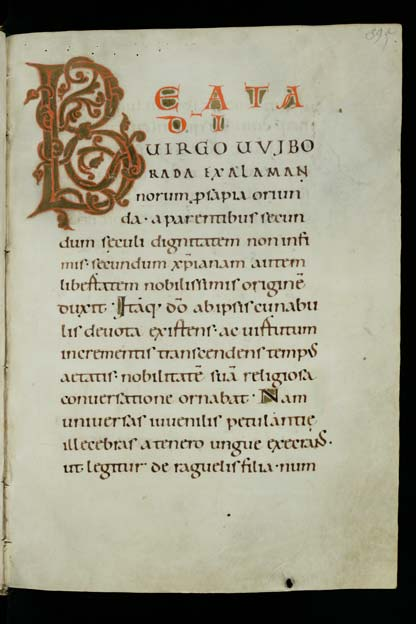
\includegraphics{img/Voigt01.jpg}
\caption{Abb. csg-0560\_395; BU/Quelle: St.~Gallen, Stiftsbibliothek,
Cod. Sang. 560, p.~395}
\end{figure}

\section*{Die erste \enquote{offizielle}
Heilige}\label{die-erste-offizielle-heilige}

Unter der Signatur Codex Sangallensis 560 verzeichnet die
Stiftsbibliothek einen Band mit den Viten dreier Heiliger -- Gallus,
Otmar und Wiborada -- aus der Zeit um 1075.\footnote{St.~Gallen,
  Stiftsbibliothek, Cod. Sang. 560: Vitae sci. Galli, sci. Otmari, scae.
  Wiboradae, \url{http://www.e-codices.unifr.ch/de/list/one/csg/0560}.}
Genau 544 Seiten feinen Kalbspergaments sind kunstvoll in karolingischer
Minuskel beschrieben. Auf den Seiten 374 bis 544 geht es um das Leben
Wiboradas -- oder Wiberat (ahd.) --, die 1047 als erste Frau von einem
Papst heiliggesprochen wurde. Der Autor, Herimannus, konnte sich auf
eine frühere Vita stützen: Kurz vor der Kanonisierung durch Clemens II.
hatte sie der damalige Leiter der Klosterschule, Ekkehart IV., verfasst
und dabei eine wiederum ältere, nicht erhaltene Vorlage verwendet, die
Ekkehart I. in den Sechzigerjahren des 10. Jahrhunderts niederschrieb,
etwa vierzig Jahre nach Wiboradas Tod 926. So weit zu den Quellen.

Wer war diese Frau, deren Name im Heiligenkalender der katholischen
Kirche unter dem 2. Mai steht?

\section*{Kulturmetropole am
Bodensee}\label{kulturmetropole-am-bodensee}

Zu Beginn des 10. Jahrhunderts bestand die Benediktinerabtei bereits
seit knapp zweihundert Jahren. Um das Kloster herum hatte sich eine
wohlhabende Ortschaft entwickelt und im Stift lebten etwa hundert
Mönche. Im weiten Umkreis war St.~Gallen bekannt als Hort der
Gelehrsamkeit, in der Schreibwerkstatt wurden die maßgeblichen
kirchlichen und wissenschaftlichen Werke kopiert und weiterverbreitet.
Die Reichsabtei mit ihrer bereits mehrere hundert Titel umfassenden
Büchersammlung bot auch das ideale Umfeld für namhafte Autoren, etwa
Notker I., zugleich Bibliothekar vor Ort (gest. 912), oder Walahfrid
Strabo (gest. 849), Abt des Klosters Reichenau und Verfasser der
\emph{Vita Sancti Galli}. St.~Gallen war ein kultureller Anziehungspunkt
ersten Ranges, als sich hier Wiborada und ihr Bruder Hitto niederließen,
beide aus adliger alamannischer Familie.

\section*{Lebendig eingemauert}\label{lebendig-eingemauert}

In den Viten wird Wiborada als Person kaum greifbar, Herkunft und
Geburtsjahr sind unbekannt. Die verschiedenen Episoden über ihr
(Nach-)Leben entsprechen den Konventionen der Zeit, in der sie
entstanden und aufgeschrieben wurden. Dennoch liefern sie ein
faszinierendes Bild einer Frauenfigur zwischen Volksglauben und
Hochkultur des Frühmittelalters.\footnote{Vgl. Karsten Uhl, \enquote{Der
  Pöbel, der nicht in gebildeten Wendungen zu sprechen versteht.}
  Unterschiede zwischen der Kultur des Volkes und der Kultur der Eliten
  in den Viten der Heiligen Wiborada, in: \emph{Volkskultur und
  Elitekultur im frühen Mittelalter}, Krems: Medium Aevum Quotidianum
  (1997), S. 103--118.}

Breiten Raum nimmt die Beziehung zu ihrem Bruder ein, mit dem sie
angeblich eine Pilgerreise nach Rom unternahm. Als er ins Kloster
eintrat, blieb sie in seiner Nähe und webte für ihn Kleidung und
Bucheinbände. Vermutlich brachte ihr Hitto das Lesen bei, denn es heißt,
er habe sie fünfzig Psalmen gelehrt, die anderen hundert hätte sie sich
mithilfe des Heiligen Geistes selbst eingeprägt. Über ihren Bruder
verschaffte sich Wiborada also Zugang zu Bildung, ein Weg, der ihr als
Frau sonst versperrt war. Sie ging noch weiter. Um 912 begann sie, mit
zwei Dienerinnen nahe dem Klosterbezirk in strenger Askese zu leben und
916 entschied sie sich, Reklusin zu werden: Sie ließ sich in einer
Klause an der Kirche St.~Mangen einmauern.

Zehn Jahre lang lebte sie in einem engen, ungeheizten Raum, eine
Maueröffnung zur Kirche hin gab den Blick auf den Altar frei, eine
zweite erlaubte den notdürftigen Austausch mit der Außenwelt. Von ihrem
spärlichen Mobiliar ist ein dreibeiniger Hocker erhalten, der heute
zusammen mit einigen Reliquien im Kloster Glattburg, 20 Kilometer
westlich von St.~Gallen, besichtigt werden kann.

In ihrer extremen Selbstkasteiung wurde Wiborada zu einem Musterbeispiel
weiblicher Frömmigkeit. Sie hatte Visionen, erteilte ihrem Namen gemäß
kluge Ratschläge, sprach Warnungen aus und machte Weissagungen. Ihr Ruf
verbreitete sich und sie zog immer mehr Gläubige an. Die Reklusin war
ein Gewinn für das Kloster.

\section*{Retterin der Bücher}\label{retterin-der-buxfccher}

In diese Zeit fielen zahlreiche Raubzüge ungarischer Reiterheere, die
vom Donaubecken weit nach Westen vordrangen und auch das Oberrhein- und
Bodenseegebiet berührten. Am 1. Mai 926 erreichte eine Truppe
St.~Gallen. Die Ungarn fanden das Kloster beinahe verlassen vor -- dafür
hatte Wiborada gesorgt. Sie warnte Abt Engilbert vor einem
bevorstehenden Überfall der Ungarn und riet ihm, Menschen, Bücher und
liturgische Schätze zu evakuieren. Bibliothek und Archiv wurden auf der
Insel Reichenau in Sicherheit gebracht, sie selbst blieb in ihrer Klause
zurück, entsprechend ihrem Gelübde.

Anscheinend verlief der Überfall glimpflich für das Kloster.\footnote{Karl
  Schmuki, \enquote{Der Einfall der Ungarn in Sankt Gallen im Jahre 926
  in den Handschriftenschätzen der Stiftsbibliothek Sankt Gallen}, in:
  \emph{Die Ungarn und die Abtei Sankt Gallen}, Sankt Gallen --
  Budapest, 1999, S. 26--36.} Doch die Reklusin wurde \enquote{von den
Heiden umgebracht}, wie das Professbuch des Klosters verzeichnet. Sie
brachen in die Klause ein und erschlugen die Bewohnerin. Als nach Abzug
der Ungarn die Mönche zurückkehrten, fanden sie die Tote und beerdigten
sie bei der Kirche St.~Mangen.

Die Bücher gerettet, das Leben verloren. Schon bald setzte eine rege
Pilgerschaft zu Wiboradas Grab ein (das heute nicht mehr lokalisierbar
ist). Die Mönche hielten ihr Andenken hoch, zahlreiche Geschichten
kursierten über sie und über angebliche Wunder an ihrem Grab. Es lag
nahe, sie aufzuschreiben und damit der Klostertradition einzugliedern.

\begin{figure}[htbp]
\centering
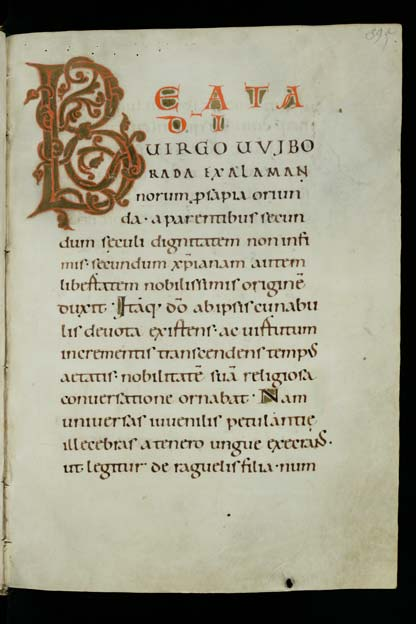
\includegraphics{img/Voigt01.jpg}
\caption{Abb. csg-0586\_230; BU/Quelle: St.~Gallen, Stiftsbibliothek,
Cod. Sang. 586, p.~230}
\end{figure}

\section*{Ausgegrenzt und
hochverehrt}\label{ausgegrenzt-und-hochverehrt}

Durch die Lebensbeschreibungen und Einträge, etwa in den Annalen, blieb
die Erinnerung an eine Frau lebendig, die ein \enquote{christliches
Tugendideal des 10. Jahrhunderts}\footnote{Eva Irblich, \enquote{Die
  Vitae Sanctae Wiboradae. Ein Heiligen-Leben des 10. Jahrhunderts als
  Zeitbild}, in: \emph{Schriften des Vereins für Geschichte des
  Bodensees und seiner Umgebung} 88, 1970, S. 185.} verkörperte. Im 15.
Jahrhundert entstand die erste bekannte Übersetzung der Herimannus-Vita
ins Deutsche. Zwischen 1430 und 1436 schrieb sie der Mönch Friedrich
Cölner in St.~Gallen auf. Das Papiermanuskript zeigt auf Seite 230 als
gerahmte, farbig ausgemalte Federzeichnung die früheste Darstellung der
Heiligen \enquote{in brauner, innen blauer Kutte mit Schleier, in der
Rechten das Buch, in der Linken die Hellebarde}.\footnote{St.~Gallen,
  Stiftsbibliothek, Cod. Sang. 586,
  \url{http://www.e-codices.unifr.ch/de/description/csg/0586}.}

Mit dem Buch als Attribut gibt Wiborada, die weise Ratgeberin, eine
wunderbare Schutzheilige für alle Bibliophilen ab. Und als Lesekundige
in einer Zeit, in der Bildung ein Privileg von Klerikern war, ist sie
ein Beispiel weiblicher Gelehrsamkeit, lange vor Hildegard von Bingen.

Aber dass sie ihren Bildungshunger nur durch Hinwendung zu äußerster
Askese und selbst gewählte Ausgrenzung stillen konnte, ausgeschlossen
von der geistig-religiösen Blüte des St.~Gallener Klosterlebens,
erscheint zynisch. Schützten die Mauern der Klause sie vor den
Anfechtungen des Lebens oder die Mönchsgesellschaft vor einer allzu
unabhängigen Frau?

Die Rettung der Bücherschätze und Wiboradas gewaltsamer Tod sind starke
Bilder im mittelalterlichen Kontext. Sie verbinden die Bibliothek als
Inbegriff abendländischer Kultur, bedroht durch die Barbaren, mit der
Weitsicht und dem Opfermut einer Außenseiterin. Es hätte eine gewisse
Logik anzunehmen, dass die Retterin nicht überleben darf.

Stoßen wir doch alljährlich am 2. Mai mit einem Glas Wiborada-Wein an,
wie er im Bistum St.~Gallen zu ihrem Gedenktag geweiht wird, und feiern
wir den freien Zugang zu Bildung und Wissen.

\section*{Literatur}\label{literatur}

Codices Electronici Sangallenses (CESG) -- Virtuelle Bibliothek,
\url{http://www.cesg.unifr.ch/de/index.htm}.

Johannes Duft, \emph{Stiftsbibliothek St.~Gallen}, St.~Gallen, 10. A.
1995.

Eva Irblich, \enquote{Die Vitae Sanctae Wiboradae. Ein Heiligen-Leben
des 10. Jahrhunderts als Zeitbild}, in: \emph{Schriften des Vereins für
Geschichte des Bodensees und seiner Umgebung} (88), 1970, S. 1--208.

Karl Schmuki, \enquote{Der Einfall der Ungarn in Sankt Gallen im Jahre
926 in den Handschriftenschätzen der Stiftsbibliothek Sankt Gallen}, in:
\emph{Die Ungarn und die Abtei Sankt Gallen}, Sankt Gallen -- Budapest,
1999, S. 26--36.

Karsten Uhl, \enquote{Der Pöbel, der nicht in gebildeten Wendungen zu
sprechen versteht.} Unterschiede zwischen der Kultur des Volkes und der
Kultur der Eliten in den Viten der Heiligen Wiborada, in:
\emph{Volkskultur und Elitekultur im frühen Mittelalter}, Krems: Medium
Aevum Quotidianum (1997), S. 103--118.

%autor
\begin{center}\rule{3in}{0.4pt}\end{center}

\textbf{Marion Voigt} M. A. hat nach der Ausbildung zur
Sortimentsbuchhändlerin Slawistik, mittelalterliche und osteuropäische
Geschichte studiert. Seit 1996 ist sie als Lektorin und Literaturagentin
selbstständig.

\end{document}
